\section{Auswertung}
\subsection{Skalierung}
Die fünf Resonanzkurven wurden bei folgenden Signalfrequenzen $\nu_e$ aufgenommen:
\begin{align*}
  \nu_{e, 1} &= \SI{10.623}{\mega\hertz} \\
  \nu_{e, 2} &= \SI{14.732}{\mega\hertz} \\
  \nu_{e, 3} &= \SI{20.555}{\mega\hertz} \\
  \nu_{e, 4} &= \SI{23.887}{\mega\hertz} \\
  \nu_{e, 5} &= \SI{29.391}{\mega\hertz}\, . \\
\end{align*}
Zu Beginn muss die Skalierungen pro Diagramm bestimmt werden. Dafür
werden die Kalibrierungspunkte, die mit Hilfe des X-Y-Schreibers aufgenommen wurden,
ausgemessen
und pro Abschnitt angegeben. Die gemessenen Wertepaare sind in Tabelle
\ref{tab:skalierung} dargestellt.

\begin{table}[H]
  \centering
\begin{tabular}{cccccccccc}

  \toprule
$\Delta{I} \, [\SI{}{\milli\ampere}]$ & $x_1 \, [\SI{}{\centi\meter}]$ &
$\Delta{I} \, [\SI{}{\milli\ampere}]$ & $x_2 \, [\SI{}{\centi\meter}]$ &
$\Delta{I} \, [\SI{}{\milli\ampere}]$ & $x_3 \, [\SI{}{\centi\meter}]$ &
$\Delta{I} \, [\SI{}{\milli\ampere}]$ & $x_4 \, [\SI{}{\centi\meter}]$ &
$\Delta{I} \, [\SI{}{\milli\ampere}]$ & $x_5 \, [\SI{}{\centi\meter}]$ \\

 \midrule
 174  & 3,45  & 177 & 3,55 & 165 & 3,35 & 182 & 3,70 & 139 & 2,75 \\
 200  & 3,05  & 183 & 3,60 & 185 & 3,65 & 185 & 3,65 & 162 & 3,15 \\
 184  & 3,15  & 181 & 3,55 & 157 & 3,10 & 136 & 2,65 & 121 & 2,35 \\
 168  & 2,75  & 185 & 3,65 & 122 & 2,30 & 144 & 2,80 & 124 & 2,40 \\
  /   &   /   & 217 & 4,30 & 120 & 2,35 & 185 & 3,65 &  /  & /    \\
  /   &   /   &   / &   /   & 155 & 3,15 & 174 & 3,50 &  /  & /    \\
  /   &   /   &   / &   /   & 124 & 2,40 & /   &  /   &  /  & /    \\
\bottomrule
\end{tabular}

\caption{Skalierung pro Abschnitt für die einzelnen Messungen}
\label{tab:skalierung}
\end{table}

Danach wird pro Diagramm die Stromstärken pro $\si{\centi\meter}$, dessen
Mittelwerte und die Fehler auf die Mittelwerte berechnet. Diese Werte sind
in Tabelle \ref{tab:procm} dargestellt.

\begin{table}
[H]
  \centering
\begin{tabular}{c|ccccc}

  \toprule
& $z_1 \, [\SI{}{\milli\ampere\per\centi\meter}]$ & $z_2 \, [\SI{}{\milli\ampere\per\centi\meter}]$ &
$z_3 \, [\SI{}{\milli\ampere\per\centi\meter}]$ & $z_4 \, [\SI{}{\milli\ampere\per\centi\meter}]$ &
 $z_5 \, [\SI{}{\milli\ampere\per\centi\meter}]$ \\

 \midrule
                    & 50,43 & 49,86 & 49,25 & 49,19 & 50,54 \\

                    & 64,52 & 50,83 & 50,68 & 50,68 & 51,43 \\

                    & 58,41 & 50,99 & 50,65 & 51,32 & 51,49 \\

                    & 61,09 & 50,68 & 53,04 & 51,43 & 50,42 \\

                    &   /   & 50,47 & 51,06 & 50,68 &   /   \\

                    &   /   &   /   & 49,21 & 49,71 &   /   \\

                    &   /   &   /   & 51,60 &   /   &   /   \\

\hline
\text{Mittelwert}   &59     & 50,6  & 50,8  & 50,5  & 51,0 \\
\text{Fehler}       & 3  & 0,2   & 0,5   & 0,4   & 0,3  \\
\bottomrule
\end{tabular}

\caption{Skalierung pro cm für die einzelnen Messungen}
\label{tab:procm}
\end{table}



\subsection{Berechnung des gyromagnetischen Verhältnisses}
Zur Bestimmung des gyromagnetischen Verhältnisses müssen zunächst die Maxima
der einzelnen Messungen lokalisiert werden. Pro Signalfrequenz sind dabei zwei
Maxima zu erkennen, eins parallel und eins antiparallel zum Erdmagnetfeld.
Ermittelt wird dabei der Abstand der jeweiligen Maxima zum Nullpunkt, welcher
dann mit der zugehören Skalierung aus Tabelle \ref{tab:procm} multipliziert
wird. Die Abstände mit den zugehörigen Stromstärken sind in Tabelle
\ref{tab:maxima} dargestellt.

\begin{table}[H]
  \centering
\begin{tabular}{c|cccc}
  \toprule
$\nu_{e, i}$ & $m_a \, [\SI{}{\centi\meter}]$ &
$I_a \, [\SI{}{\milli\ampere}]$ & $m_p \, [\SI{}{\centi\meter}]$ &
$I_p \, [\SI{}{\milli\ampere}]$ \\
 \midrule
  $\nu_{e, 1}$ & 4,35 & 250 \pm 10  & 3,20  &  190  \pm 10 \\
  $\nu_{e, 2}$ & 8,00 & 405 \pm 2 & 6,80   &  344 \pm 1 \\
  $\nu_{e, 3}$ & 11,00 & 559 \pm 6 & 9,70   &  493 \pm 5 \\
  $\nu_{e, 4}$ & 12,25 & 619 \pm 4 & 11,20  &  566 \pm 4 \\
  $\nu_{e, 5}$ & 14,90 & 759 \pm 4 & 13,85  &  706 \pm 4 \\
\bottomrule
\end{tabular}
\caption{Lokalisierung der Maxima mit den zugehörigen Stromstärken pro
Signalfrequenz}
\label{tab:maxima}
\end{table}


Zur Berechnung des gyromagnetischen Verhältnisses wird die Stärken der jeweiligen
Magnetfelder benötigt. Diese lassen mit Hilfe von Formel \eqref{eqn:B}
berechnen. Die dabei verwendeten Konstanten \cite{skript} \cite{indu} lauten
\begin{align*}
  n &= 156 \\
  r &= \SI{0.1}{\meter} \\
  \mu_0 &= 4 \pi \cdot 10^{-7}\, \si{\volt\second\per\ampere\per\meter} \, .\\
\end{align*}

Der Fehler wird mit

\begin{equation}
  \Delta{B} = \frac{8}{\sqrt{125}} \mu_0 \frac{n}{r} \Delta{I}
\end{equation}

berechnet.

Die parallel und antiparallel zum Erdmagnetfeld ausgerichteten Magnetfeldstärken
sind mit ihrer zugehörigen Signalfrequenz in Tabelle \ref{tab:bfelder} dargestellt.

\begin{table}[H]
  \centering
\begin{tabular}{c|ccc}
  \toprule
$\nu_{e, i}$ & $B_a \, [\SI{}{\micro\tesla}]$ &
$B_p \, [\SI{}{\micro\tesla}]$ & $\bar{B} \, [\SI{}{\micro\tesla}]$ \\
 \midrule
  $\nu_{e, 1}$ & 357,145 & 258,871 & 308,008    \\
  $\nu_{e, 2}$ & 567,482 & 482,366 & 524,924    \\
  $\nu_{e, 3}$ & 783,529 & 690,935 & 737,232    \\
  $\nu_{e, 4}$ & 867,762 & 793,376 & 830,569   \\
  $\nu_{e, 5}$ & 1065,292 & 990,219 & 1027,756  \\
\bottomrule
\end{tabular}
\caption{Zu den Signalfrequenzen zugehörigen berechneten Magnetfelder}
\label{tab:bfelder}
\end{table}


Aus Formel \eqref{eqn:hv}
kann der folgende Zusammenhang entnommen werden

\begin{equation}
  B = \frac{h \nu_e}{g \mu_B} \, .
\end{equation}

Um das gyromagnetische Verhältnis zu bestimmen, wird diese Formel in eine
Gleichung der Form

\begin{align*}
  f(x) = ax + b
\end{align*}
umgeformt. Daraus folgt die Funktion

\begin{align*}
  B(\nu_e) = \frac{h}{g \mu_B} \cdot \nu_e + b \, .
\end{align*}

Aus der Steigung kann dann das gyromagnetische Verhältnis berechnet werden.
Die Messwerte und die Ausgleichsfunktion sind in Abbildung \ref{fig:plot}
dargestellt.

\begin{figure}[H]
  \centering
  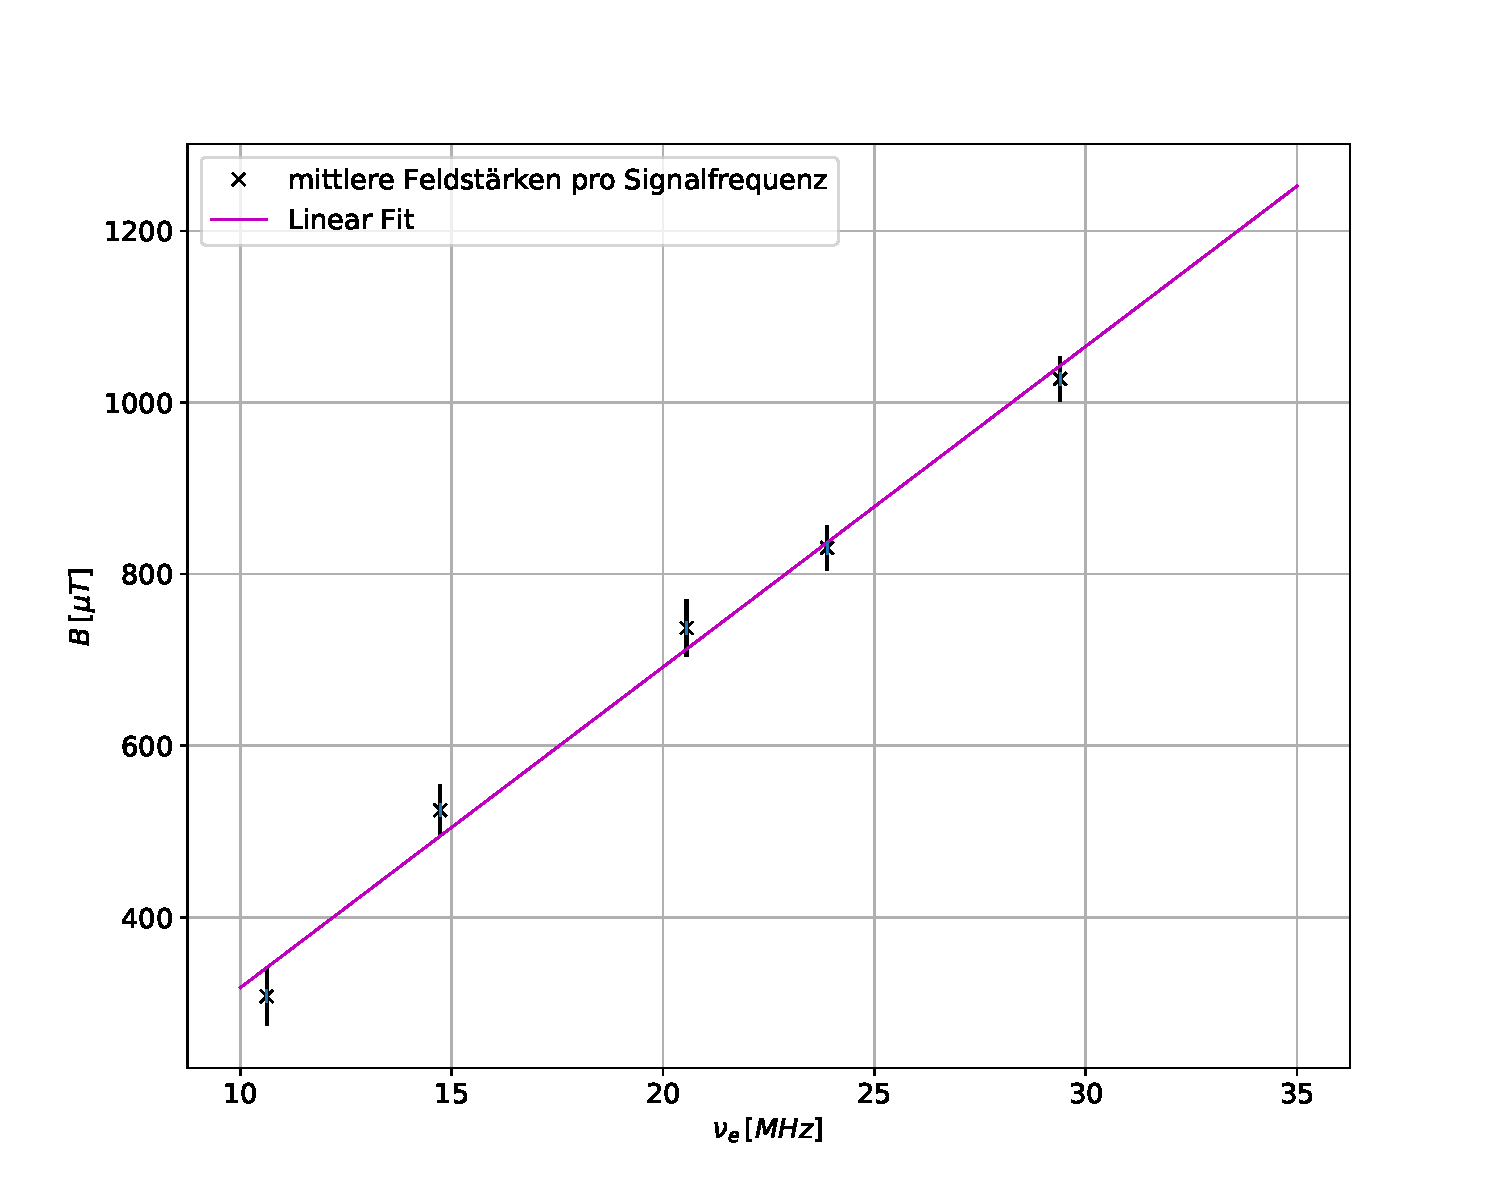
\includegraphics[width=\textwidth]{plot.pdf}
  \caption{Ausgleichsfunktion zur Bestimmung des gyromagnetischen Verhältnisses}
  \label{fig:plot}
\end{figure}

Die Parameter der Ausgleichsfunktion lauten

\begin{align*}
  a = \frac{h}{g \mu_B} &= \SI{37.38 \pm 2.10}{\micro\tesla\per\mega\per\hertz} \\
  b & = \SI{-55.88 \pm 43.84}{\micro\tesla} \, .
\end{align*}

Das gyromagnetische Verhältnis berechnet sich dann durch
\begin{equation}
  g = \frac{h}{a \mu_B} \, .
\end{equation}

Der Fehler berechnet sich mit Hilfe der Gaußschen Fehlerfortpflanzung, also mit

\begin{align*}
\Delta{g} = - \frac{h}{a^2 \mu_B} \Delta{a} \, .
\end{align*}

Das gyromagnetische Verhältnis des freien Elektrons lautet demnach

\begin{align*}
  g = \SI{1.9 \pm 0.1}{} \, .
\end{align*}

\subsection{Bestimmung des Erdmagnetfelds am Messort}
Zur Bestimmung des Erdmagnetfeldes werden die berechneten Magnetfeldstärken
aus Tabelle \ref{tab:bfelder} erneut benötigt. Unter der Annahme, dass das
Erdmagnetfeld eine gegensätzliche Verschiebung der Resonanzkurven für ein
paralleles und antiparalleles Feld bewirkt, kann auf die Folgende Gleichung
geschlossen werden

\begin{equation}
  B_{\text{Erd}} = \frac{B_a - B_p}{2} \, .
\end{equation}

Dadurch ergeben sich die in Tabelle \ref{tab:erde} dargestellten Erdmagnetfeldstärken.
Der Fehler berechnet sich durch
\begin{align*}
  \Delta{B_{\text{Erd}}} = \sqrt{\Delta{B_a}^2 + \Delta{B_p}^2} \, .
\end{align*}

\begin{table}[H]
  \centering
\begin{tabular}{cc}
  \toprule
$\nu_{e, i}$ & $B_{\text{Erd}} \, [\SI{}{\micro\tesla}]$ \\
 \midrule
  $\nu_{e, 1}$ & 98,27 \pm 22,72 \\
  $\nu_{e, 2}$ & 85,12 \pm 2,94 \\
  $\nu_{e, 3}$ & 92,59 \pm 10,28\\
  $\nu_{e, 4}$ & 74,39 \pm 8,38 \\
  $\nu_{e, 5}$ & 75,07 \pm 7,99 \\
\bottomrule
\end{tabular}
\caption{Pro Signalspannung und Resonanzkurve berechnete Erdmagnetfeldstärken}
\label{tab:erde}
\end{table}

Die mittlere Erdmagnetfeldstärke mit dem Fehler auf dem Mittelwert betragen
dann

\begin{align*}
 B_{\text{Erd}} = \SI{43 \pm 5}{\micro\tesla}
\end{align*}
